\documentclass{article}

% Encoding
\usepackage[utf8]{inputenc}
% Little tweaks for the margins
\usepackage[margin=2.5cm]{geometry}
% Including graphics
\usepackage{graphicx}

\title{LINFO1252 : Système Informatique}
\author{Nathan Tihon}
\date{\today}

\begin{document}

\begin{titlepage}
  \begin{sffamily}
  \begin{center}

    % École
    ~\\[0.5cm]\textsc{\LARGE Université catholique de Louvain}\\[0.5cm]
    %Ou 
    
    % Cours
    \textsc{\Large LINFO1252 - Systèmes Informatiques }\\[2cm]
    

    % Titre
    \HRule \\[0.7cm]
    \textbf{ \huge Evaluation de performances d'algorithmes de synchronisation } \\[4mm]
    \Large{Année académique 2021-2022} \\[2mm]
    \large{Date de soumission : \ 7 décembre 2021}
    \HRule \\[2cm]
    
    \begin{center}
        
\includegraphics[scale=0.65]{img/epl-logo.jpg}
    \end{center}
    \vspace{2cm}
    \begin{minipage}{1.0\textwidth}
      \begin{center} \large
        Nathan \textsc{Tihon} \\[0.1cm]
        Noma : \textsc{10851900}\\
        \vspace{0.5cm}
        \textsc{Tuteur :} \\[0.1cm]
        Jonathan \textsc{de Salle}
        \vspace{0.5cm}
        
        \textsc{Professeur:}\\[0.1cm]
         Etienne \textsc{Rivière} \\
      \end{center}
    \end{minipage}
    \\[0.3cm]

    % Bas de page
    \vfill
{\large }%date ou autre
  \end{center}
  \end{sffamily}
\end{titlepage}

\newpage

\section{Introduction}

Le but de ce projet est d'implémenter et évaluer les performances de plusieurs algorithmes de synchronisation.
L'évaluation de performances ayant été effectuée s'articule autour de 2 paramètres, le nombre de \textit{thread} et le type de primitive de synchronisation utilisées.
Le nombre de thread sera un paramètre entier comprit entre 1 et $2n$ où $n$ est le nombre de coeurs du processeur \footnote{Le processeur utilisé dans le cadre de ces tests est un Intel i5 9400f, dont les informations techniques peuvent être retrouvées ici :https://www.intel.fr/content/www/fr/fr/products/sku/190883/intel-core-i59400f-processor-9m-cache-up-to-4-10-ghz/specifications.html?wapkw=9400F } tandis que les primitives utilisées appartiendront quant à elle à 2 catégories. La première comprend les mutex et sémaphores POSIX provenant de \texttt{<pthread.h>} et de \texttt{<semaphore.h>} alors que la seconde englobe les verrous à attente active (spinlock) ainsi que les sémaphores construites sur ces verrous.\\ 

\noindent Les figures analysées dans ce rapport seront composées de 2 courbes représentant le temps moyen en fonction du nombre de threads, accompagnées de "barres d'erreur" représentant l'écart-type des mesures.
Les couleurs représentent la catégorie de primitives utilisées (paramètre catégoriel), l'axe des abscisses montre le nombre de thread (paramètre entier) et l'axe des ordonnées représente le temps d'exécution en fonction de ces paramètres. \\

\noindent Il est à noter qu'à partir de la section 3 les figures présentent toutes une valeur nulle pour un thread unique. Cela est dû au fait que nous analysons des algorithmes de \textit{synchronisation}.
Il nous faut donc au minimum 2 threads pour pouvoir analyser le comportement de ces algorithmes. Une autre information importante pour la bonne compréhension du lecteur est le fait que je parle très souvent de \textit{compétitivité au niveau des mutex}. J'entend par cela que plusieurs threads tentent d'accéder à un mutex de manière concurrente et/ou répétée.

\section{Verrous à attente active}

Commençons tout d'abord par analyser la performance des spinlocks, car nous utiliseront ceux-ci dans la suite de nos analyses. Il est ici proposé de comparer
2 algorithmes d'implémentation de spinlocks : l'algorithme \textit{test-and-set}, et l'algorithme \textit{test-and-test-and-set} \footnote{Ces algorithmes sont nommées TAS et TATAS pour la suite de ce rapport}, j'ai prit la liberté d'également afficher les performances des mutex POSIX afin d'avoir un témoin. La figure (\ref{pic:spinlock}) représente les performances des spinlocks.\\

\begin{figure}[h]
    \centering
    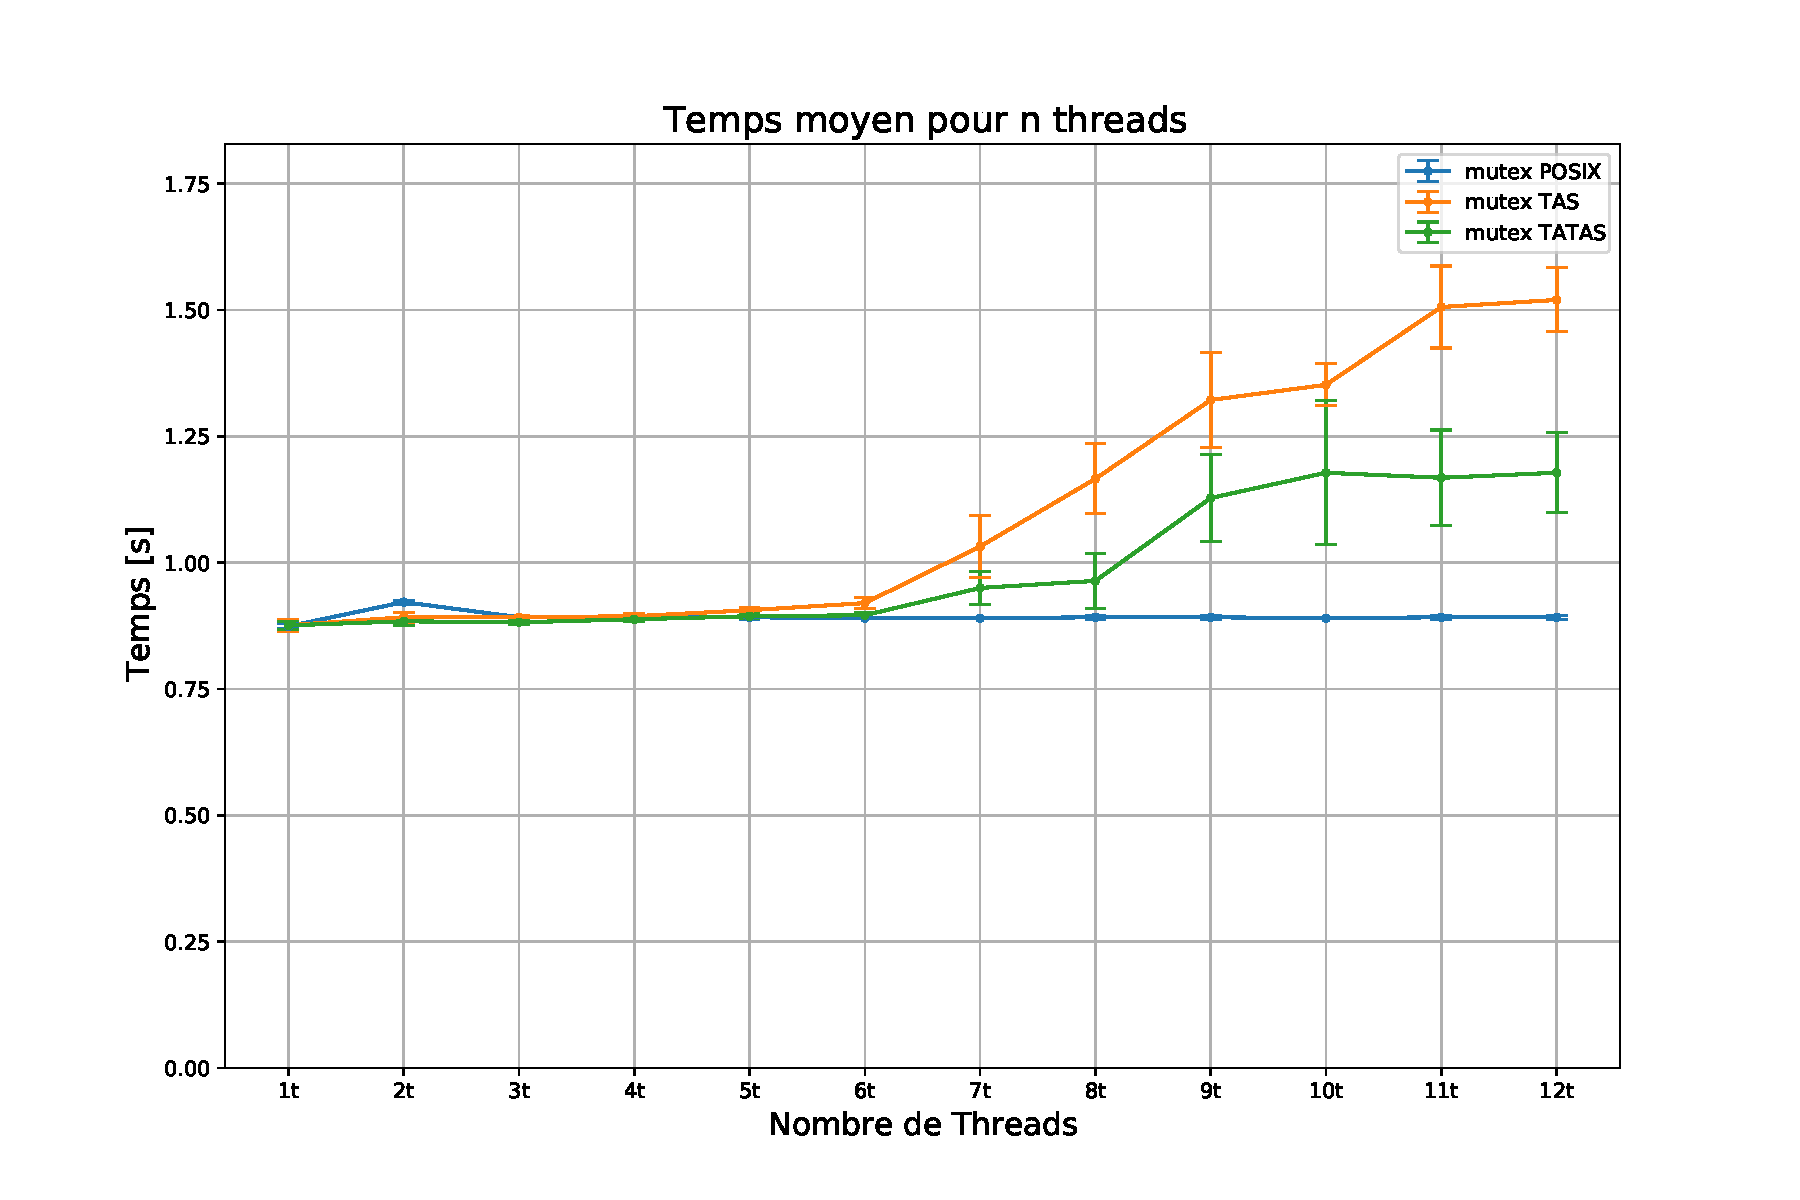
\includegraphics[scale=0.4]{img/spinlock.pdf}
    \caption{Temps d'exécution d'un spinlock dans différentes conditions}
    \label{pic:spinlock}
\end{figure}

\noindent Nous pouvons observer que les performances des 3 types de mutex sont semblables et stables jusqu'au seuil de 6 threads, à partir duquel les performances divergent.
On peut ensuite observer que les performances de l'algorithme TAS se dégradent plus vite que celles de l'algorithme TATAS lorsque l'on augmente le nombre de threads. \\

\noindent La stabilité des performances jusqu'à 6 threads peut être expliquée par 2 phénomènes. Le premier étant qu'il n'est pas nécessaire d'effectuer de changements de contexte intra-processus pour terminer l'algorithme. Le second étant le fait que dans cet algorithme les threads ne partagent pas de variables globales à l'exception du mutex. Cela signifie que les appels répétés aux instructions \texttt{xchg} n'impactent pas la vitesse de travail du thread se trouvant dans sa section critique.\\[0.1cm]

\noindent A partir de 7 threads néanmoins, les changements de contextes deviennent obligatoires. Cela peut impacter la performance de plusieurs manières. La première provient du fait que comme les spinlocks ne sont pas implémentés au niveau du noyaux, le scheduler peut décider de préempter un thread se situant dans sa section critique. Ce qui empêcherait donc le programme d'avancer dans son travail. Le second impact provient du fait que les changements de contextes devront toujours s'effectuer lors de l'exécution d'instructions \texttt{xchg}. Or un changement de contexte nécessite la restauration des variables globales du thread ainsi que des ses registres \texttt{\%esp, \%eip}, ce qui ne peut s'effectuer parallèlement aux instructions atomiques car celles-ci provoquent un blocage du bus de cache.

\noindent Au vu des meilleures performances des mutex TATAS, j'ai choisi d'implémenter les sémaphores sur base de ceux-ci.
\section{Problème des philosophes}

\begin{figure}[H]
    \centering
    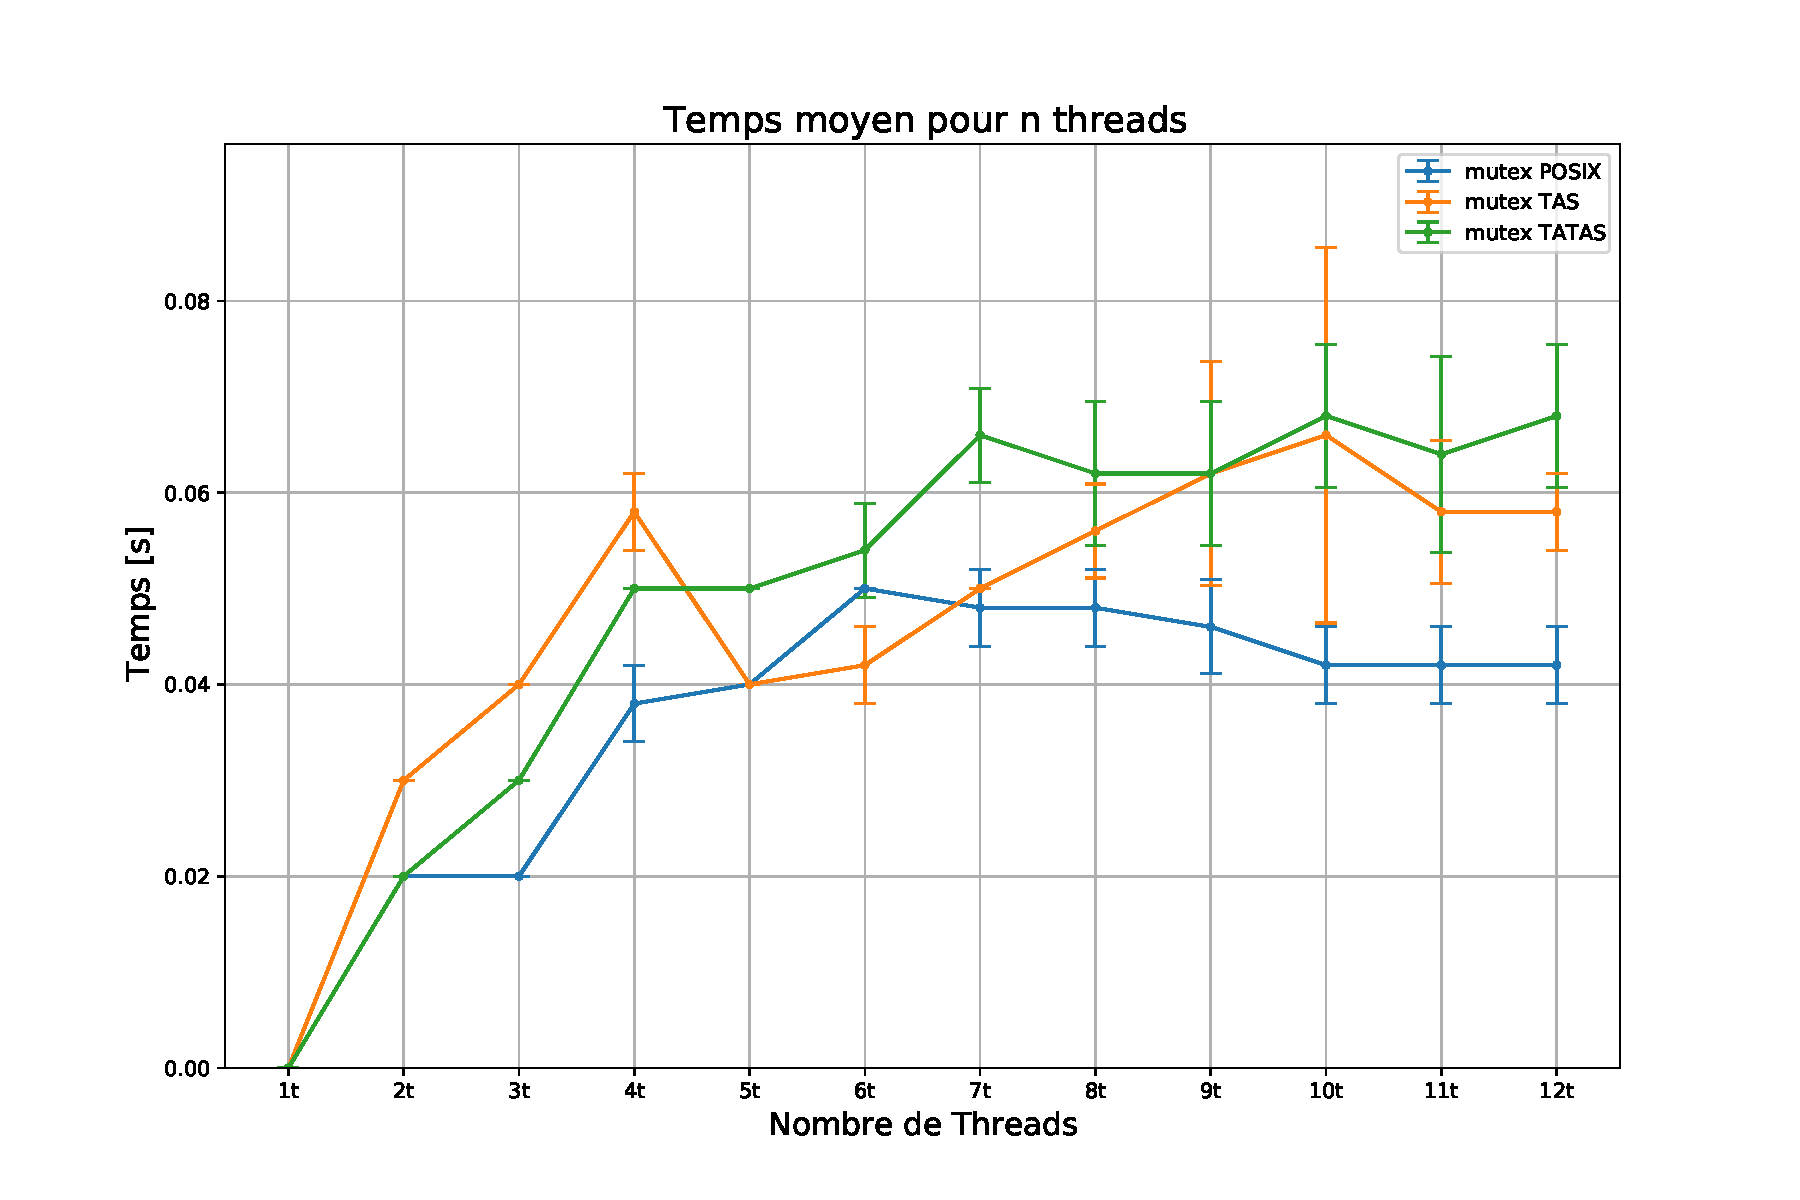
\includegraphics[scale=0.4]{img/philosophes.pdf}
    \caption{Temps d'exécution du problème des philosophes dans différentes conditions}
    \label{pic:philo}
\end{figure}

\noindent On observe que les deux courbes commencent par une phase de croissance pour se terminer par une phase de stabilisation.
On observe également que les mutex POSIX sont généralement plus stable que les spinlock TATAS. En effet on voit clairement que l'écart-type est bien inférieur. \\

\noindent Nous savons que théoriquement, le temps d'exécution est censé être constant. En effet, $n$ threads effectuant un travail équivalent \textit{parfaitement} en parallèle devraient terminer en même temps. Ce n'est évidemment pas le cas, il y a donc une perte de performances dûe à la synchronisation.\\

\noindent On peut expliquer la croissance initiale rapide par le fait que comme il y a peu de threads -et donc peu de mutex- les threads sont constamment en "combat" pour les mutex car ils peuvent tous se trouver en état Running simultanément. Il y'a donc une grosse perte de performance.\\

\noindent Par contre, lorsque le nombre de thread augmente il devient impossible de retrouver tous les threads en état Running simultanément. Cela devrait donc signifier une augmentation encore plus forte du temps d'exécution car il devient impossible d'exécuter tous les threads simultanément (et il y a donc un travail effectif plus grand). Or on remarque une stabilisation entre 6 et 12 threads. Cela peut être expliqué par le fait que la compétitivité au niveau des mutex est amoindries. En effet, comme il ne devient plus possible pour tous les threads de s'exécuter en même temps, certains threads en cours d'exécution pourront avoir accès à leurs deux mutex respectifs sans encombres. On peut tout de même raisonnablement supposer que le gain de temps découlant de la perte de compétitivité ne permettra pas de compenser l'augmentation du temps dû à l'augmentation du travail effectif indéfiniment. C'est à dire qu'on peut faire l'hypothèse que la fonction du temps d'exécution en fonction du nombre de threads deviendra monotonement croissante à partir d'une quantité seuil de threads.\\

\noindent Pour finir, on remarque que les spinlocks sont mois performants que les mutex POSIX. Cela est cohérent avec ce que l'on a vu au cours : l'attente active est moins efficace lorsque le temps d'exécution d'une section critique (SC) est plus petit ou égal aux temps entre 2 accès à cette SC, ce qui est le cas pour cet algorithme.

\section{Problème des Producteurs-Consommateurs}

\begin{figure}[H]
    \centering
    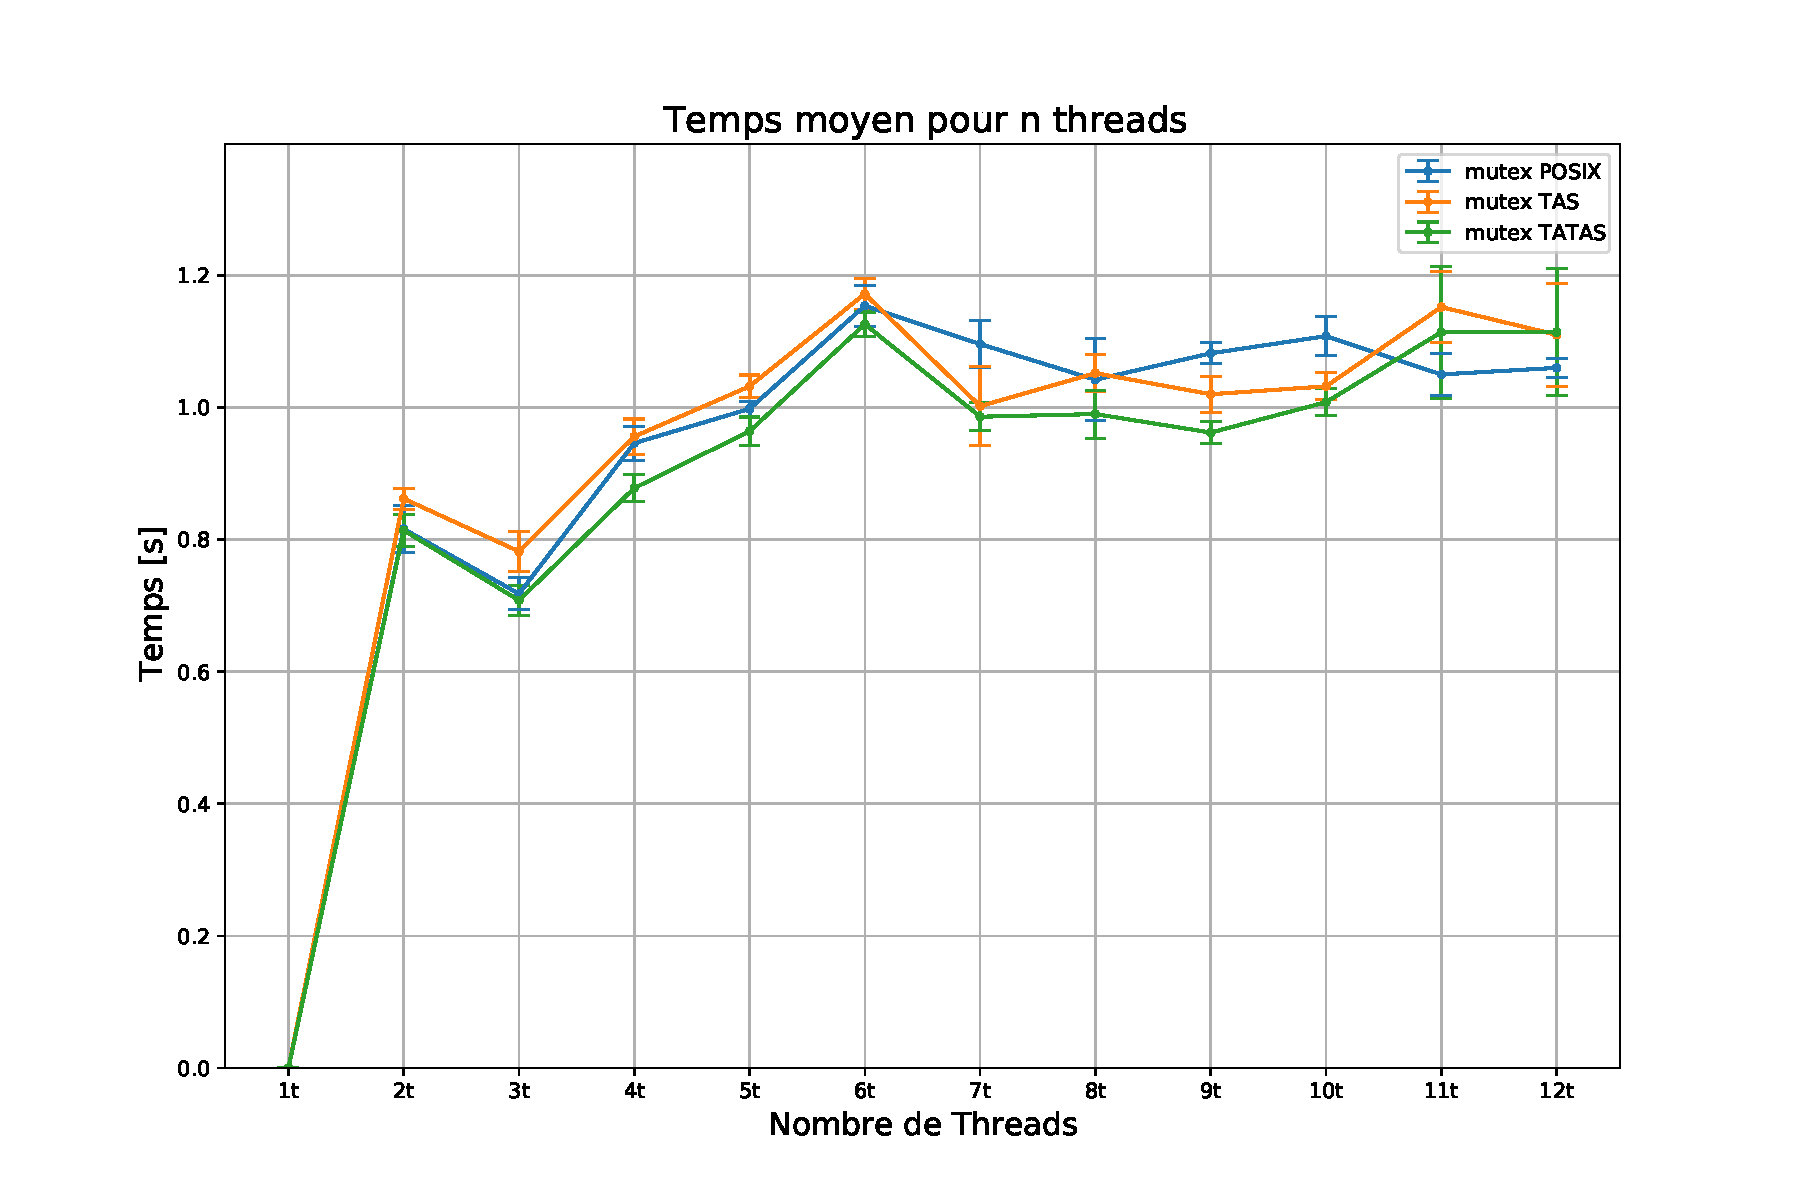
\includegraphics[scale=0.45]{img/prodcons.pdf}
    \caption{Temps d'exécution du problème des producteurs-consommateurs dans différentes conditions}
    \label{pic:prodcons}
\end{figure}

\noindent La chose importante à remarquer dans ce graphe est le fait que les courbes ne divergent pas, elles sont constamment proches. Cela peu être expliqué par le fait que contrairement au problème des philosophes, le temps entre deux accès à la SC est ici beaucoup plus long que le temps d'exécution de celle-ci. On a en effet vu au cours que l'attente active est efficace dans ces conditions car il n'est pas nécéssaire d'effectuer de changement de contexte lorsqu'un mutex se libère, un thread bouclant sur le mutex peut directement se l'approprier et entrer dans sa section critique.\\

\noindent On peut ensuite remarquer une croissance de 2 à 6 threads et une stabilisation au delà de 6 threads. Ce n'est pas vraiment à cela que je m'attendais, j'attendais plutôt une décroissance de 2 à 6 threads, étant donné que le travail est divisé au sein de plusieurs threads. La seule hypothèse me permettant de justifier le comportement observé est que le temps de processing n'est pas suffisant et il y a donc une compétitivité au niveau des mutex qui engendre une réduction de performance. Si On suppose un temps de processing (préparation et consommation de données) très long, on peut raisonnablement penser que la compétitivité au niveau des mutex sera faible et donc qu'un tel algorithme s'approcherait d'un algorithme de synchronisation parfait, signifiant que les threads effectuent effectivement leurs travail en parallèle. \\

\noindent La stabilisation au delà de 6 threads peut quant à elle être expliquée par le fait qu'il devient impossible pour le processeur d'exécuter tous les threads en même temps. Ajouter plus de threads n'augmentera donc plus la compétitivité au niveau des mutex. Les changements de contextes ne permettent pas d'augmenter considérablement le temps d'exécution dans le cas de cet algorithme car ils deviennent négligeables par rapport au temps entre deux SC.


\section{Problème des lecteurs-écrivains}

\begin{figure}[H]
    \centering
    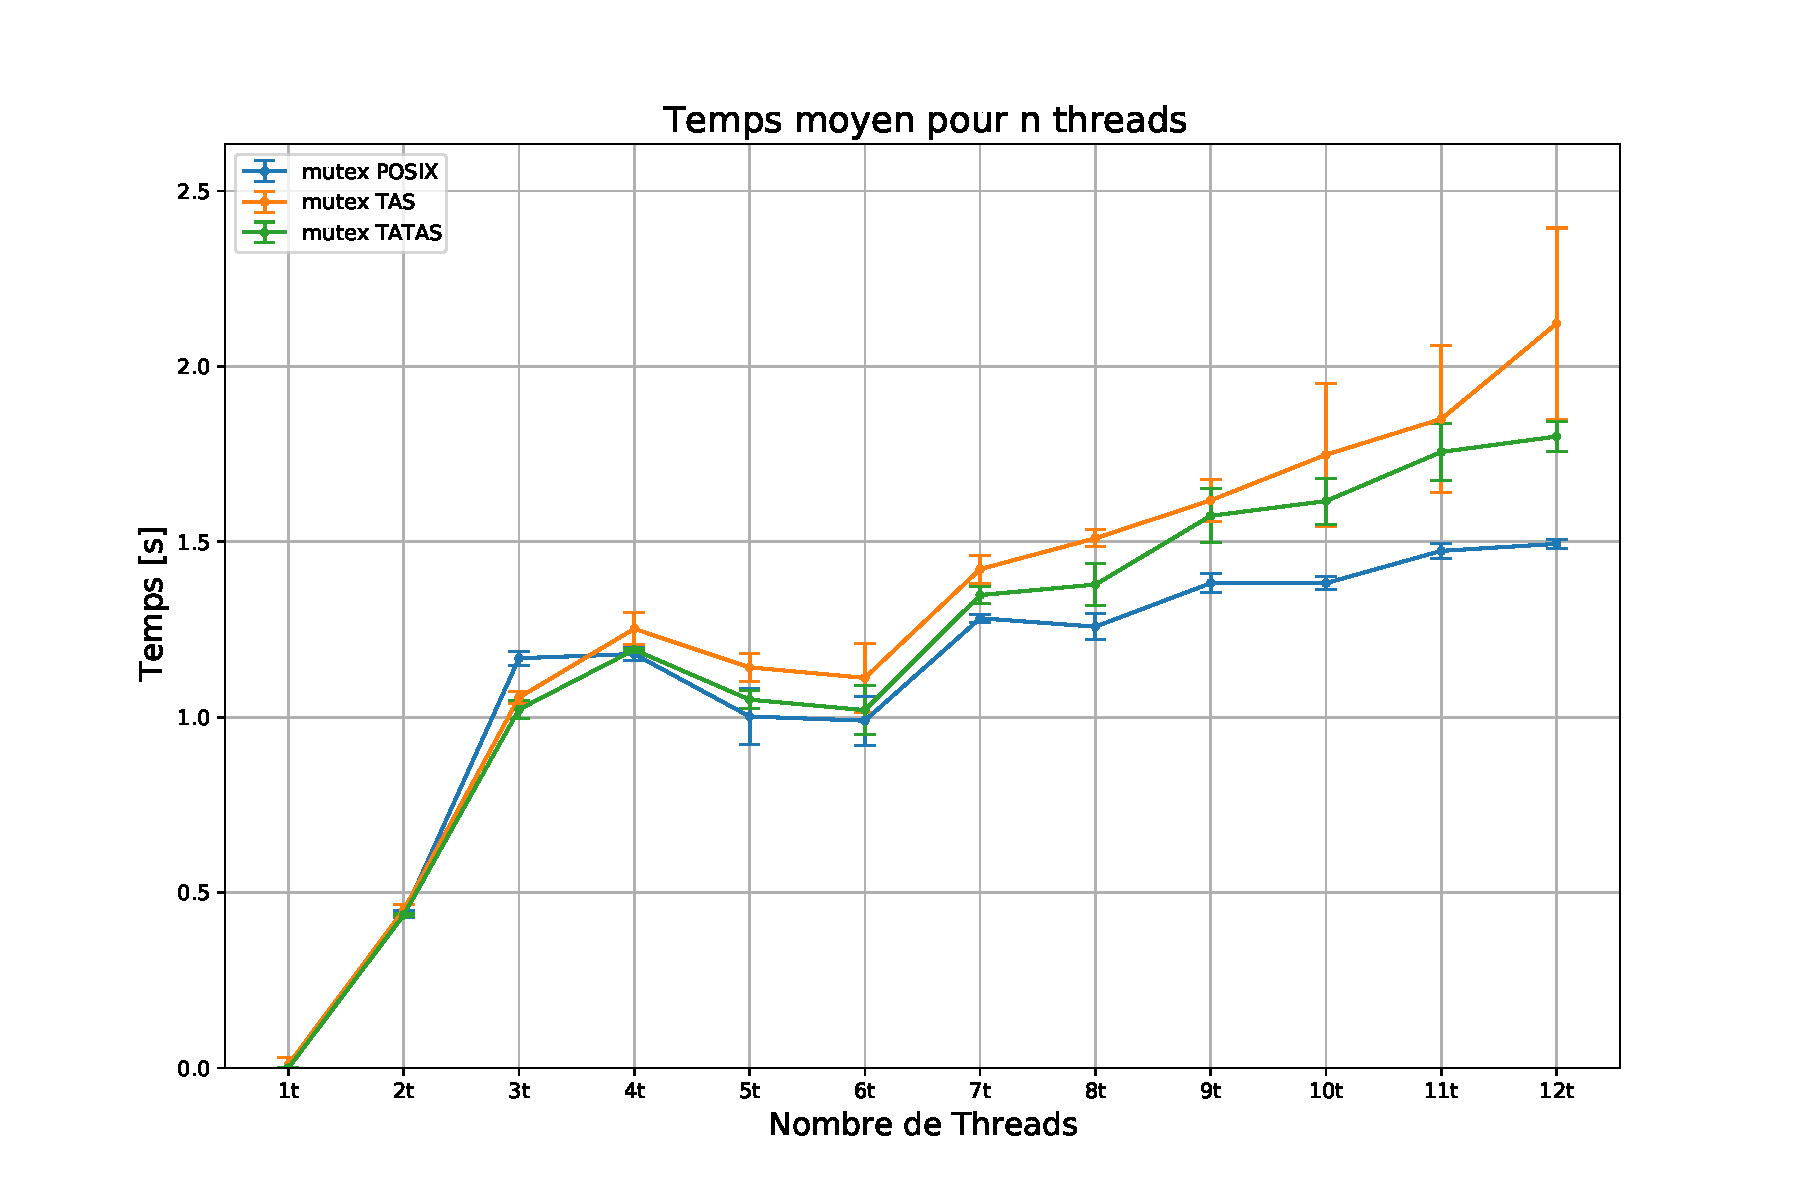
\includegraphics[scale=0.45]{img/readwrt.pdf}
    \caption{Temps d'exécution du problème des lecteurs-écrivains dans différentes conditions}
    \label{pic:readwrt}
\end{figure}

\noindent Il y a plusieurs choses intéressantes à remarquer sur ce graphique. La première étant que le graphe est composé de "marches", c'est à dire que passer d'un nombre impair de threads au nombre pair directement supérieur n'a que très peu d'impact sur le temps d'exécution. La seconde étant le creux au niveau des threads 5 et 6. Nous pouvons ensuite observer une croissance constante du temps d'exécution à partir de 6 threads. Finalement la dernière observation concerne la divergence des deux courbes à partir de 7 threads.\\

\noindent La première observation peut être expliquée par le fait que passer d'un nombre pair de threads au nombre impair directement supérieur à pour effet d'ajouter un \textit{écrivain}. Or nous savons que dans cet algorithme, seul un écrivain peut se trouver en section critique simultanément. Ajouter un écrivain ne produit donc pas plus de compétitivité au niveau des mutex, il n'y a donc que très peu de pertes de performances due à l'augmentation du travail de synchronisation d'un écrivain supplémentaire.\\

\noindent Le creux au niveau des threads 5 et 6 peut être expliqué par le fait que nous arrivons au maximum de threads simultanément exécutable pas le processeur. Il ne sera donc pas nécessaire d'effectuer de changements de contextes pour atteindre la fin de l'exécution de l'algorithme. De plus, plus de lecteurs simultané signifie que le nombre total de lectures s'effectue plus rapidement.\\

\noindent La croissance à partir de 6 threads peut s'expliquer par le simple fait qu'il devient nécessaire d'effectuer des changements de contextes en plus de la synchronisation. Et la divergence à partir de ce seuil peut être expliquée de la même manière que la divergence au niveau du problème des philsophes, l'attente active est moins efficace lorsque le temps d'accès entre deux SC est plus petit ou égal au temps d'exécution de cette SC.

\section{Conclusion}

D'un point de vue théorique, j'ai pu apprendre lors de ce projet qu'ajouter des threads n'est pas synonyme d'amélioration de performances.
En effet, j'ai pu voir qu'il est nécessaire de prendre en compte le temps d'exécution des sections critiques ainsi que le temps entre 2 accès à celles-ci. 
J'ai également pu apprendre à effectuer des instructions atomiques en assembleur, tout en prenant conscience de l'impact de ces instructions sur les performances \textit{générales} de l'ordinateur. 
L'écriture d'opération en assembleur m'a également permis d'en apprendre davantage sur la gestion des registres des processeurs et les interactions de ces derniers avec le bus de cache. \\

\noindent D'un point de vue pratique, je me suis forcé à écrire du code propre et \textit{générique}. Ce qui m'a permit de découvrir l'utilité des unions afin d'écrire des interfaces facilement utilisables avec des types de données différentes. \\

\noindent En conclusion, ce projet m'a permit d'ouvrir les yeux sur le point de vue \textit{hardware} du multithreading tout en améliorant mes capacités d'écriture et d'analyse de code nécéssaire à tout programmeur.


\end{document}

